\chapter{LHC-ATLAS実験}
\label{chap_TGC}

% この章では、自分の研究に関連する分野の歴史や現状について説明したり、研究を展開する上で重要となる知識の解説を行います。ここで使用している見出し「ガンマ線天文学…」はあくまで例ですが、もしCherekov Telescope Array(CTA)計画\footnote{省略語は必ず正式名称を先に書き、省略系は丸括弧に入れます。省略語はあくまで「以降このように略す」という用途だからです。また、日本語文章中で使う丸括弧は()ではなく()です。}に携わる院生の書く修士論文であれば、ガンマ線天文学や宇宙線物理学全般について、現行望遠鏡とガンマ線観測の原理について、またCTA計画についての記述がこの章では期待されます。

% 場合によっては「序論」と合体させても良いですが、本章は比較的長くなり結論に直結しない情報もたくさん出てくるため、独立した章である方が読者は読みやすいでしょう。

% またこの章が長くなるときには、例えば「ガンマ線天文学」と「CTA計画」のように、2つの章に分割するというのも良いと思います。\footnote{注意書きの練習です。}


\section{ATLAS検出器}
\label{sec_ATLAS}


\begin{figure} 
\centering
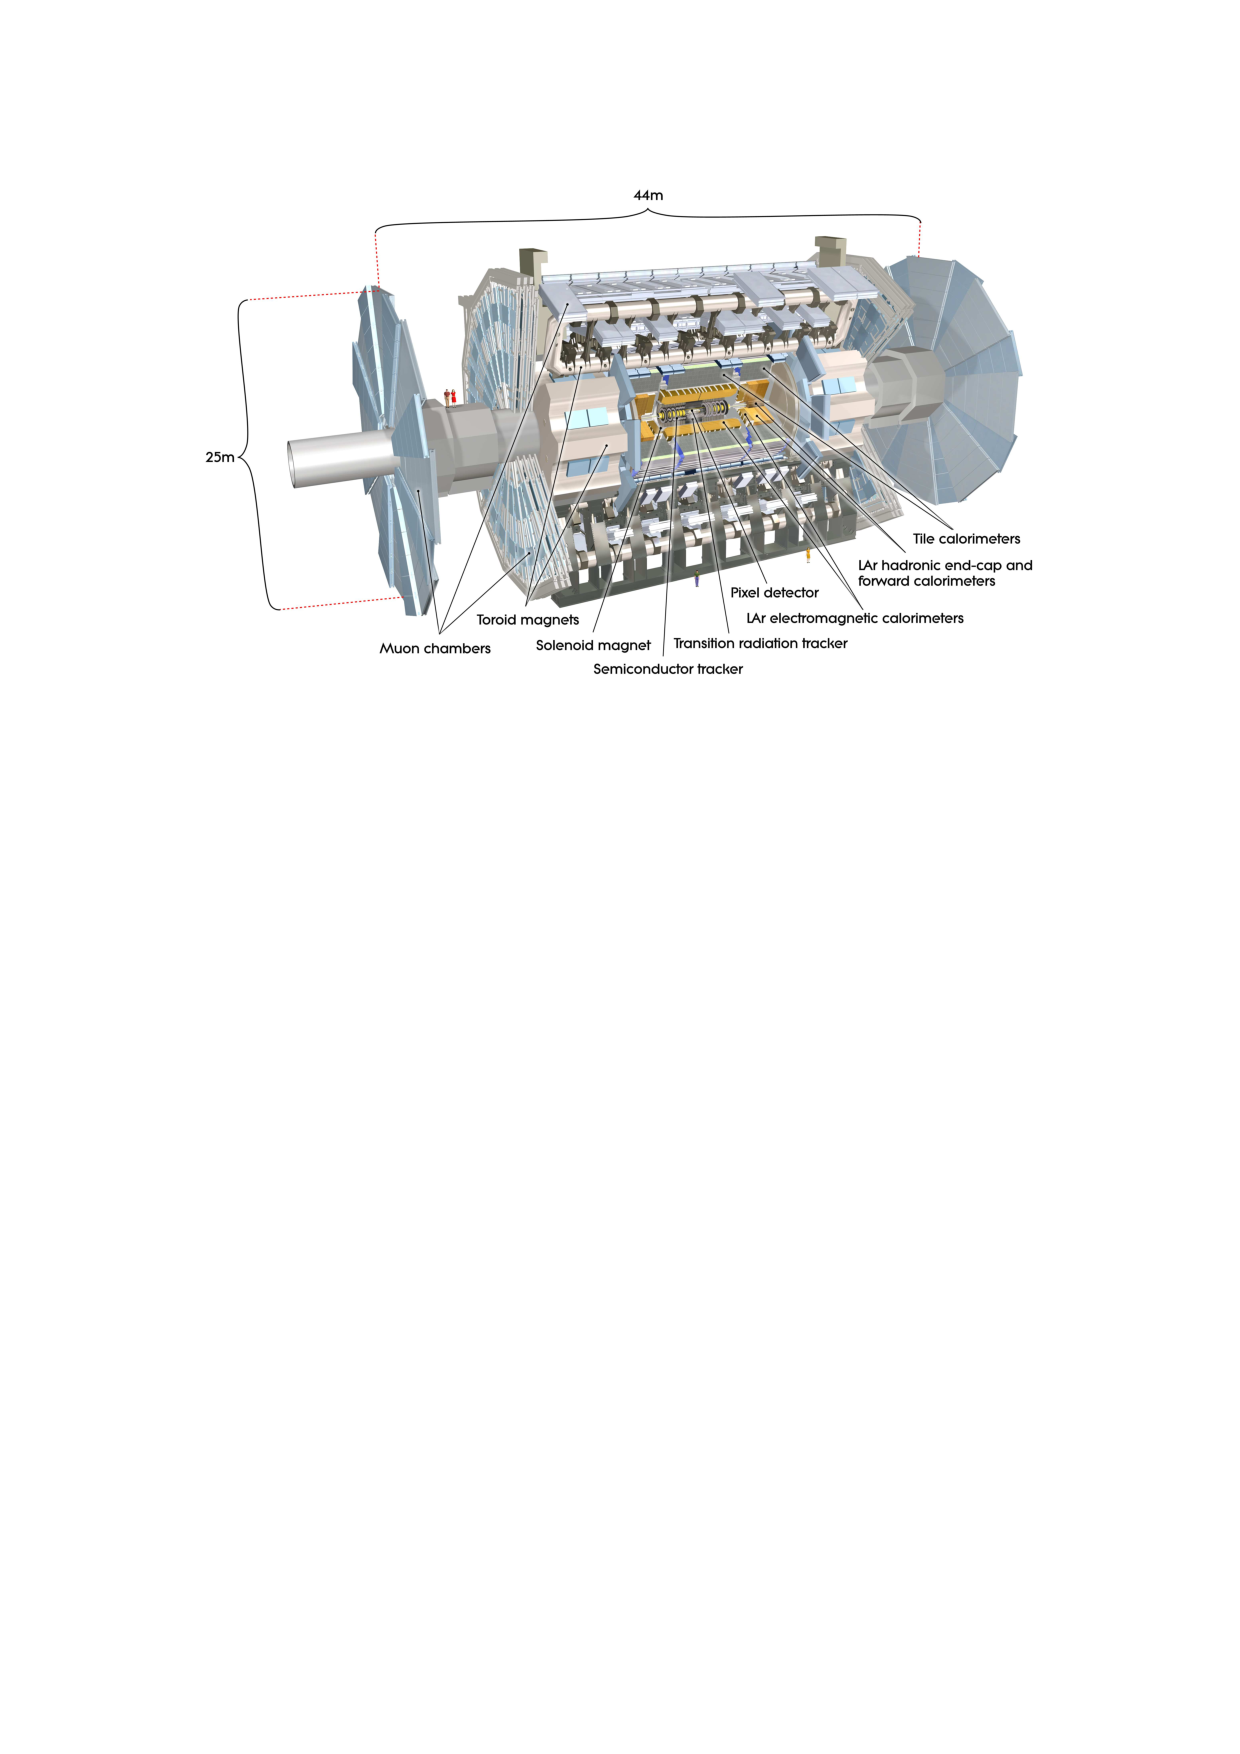
\includegraphics[width=16cm]{fig/Intro/ATLASdetector.pdf}
\caption[ATLAS検出器の概要]{ATLAS検出器の概要図\cite{JINST:2008}}
\label{ATLASdetector2}
\end{figure}

\begin{figure} 
\centering
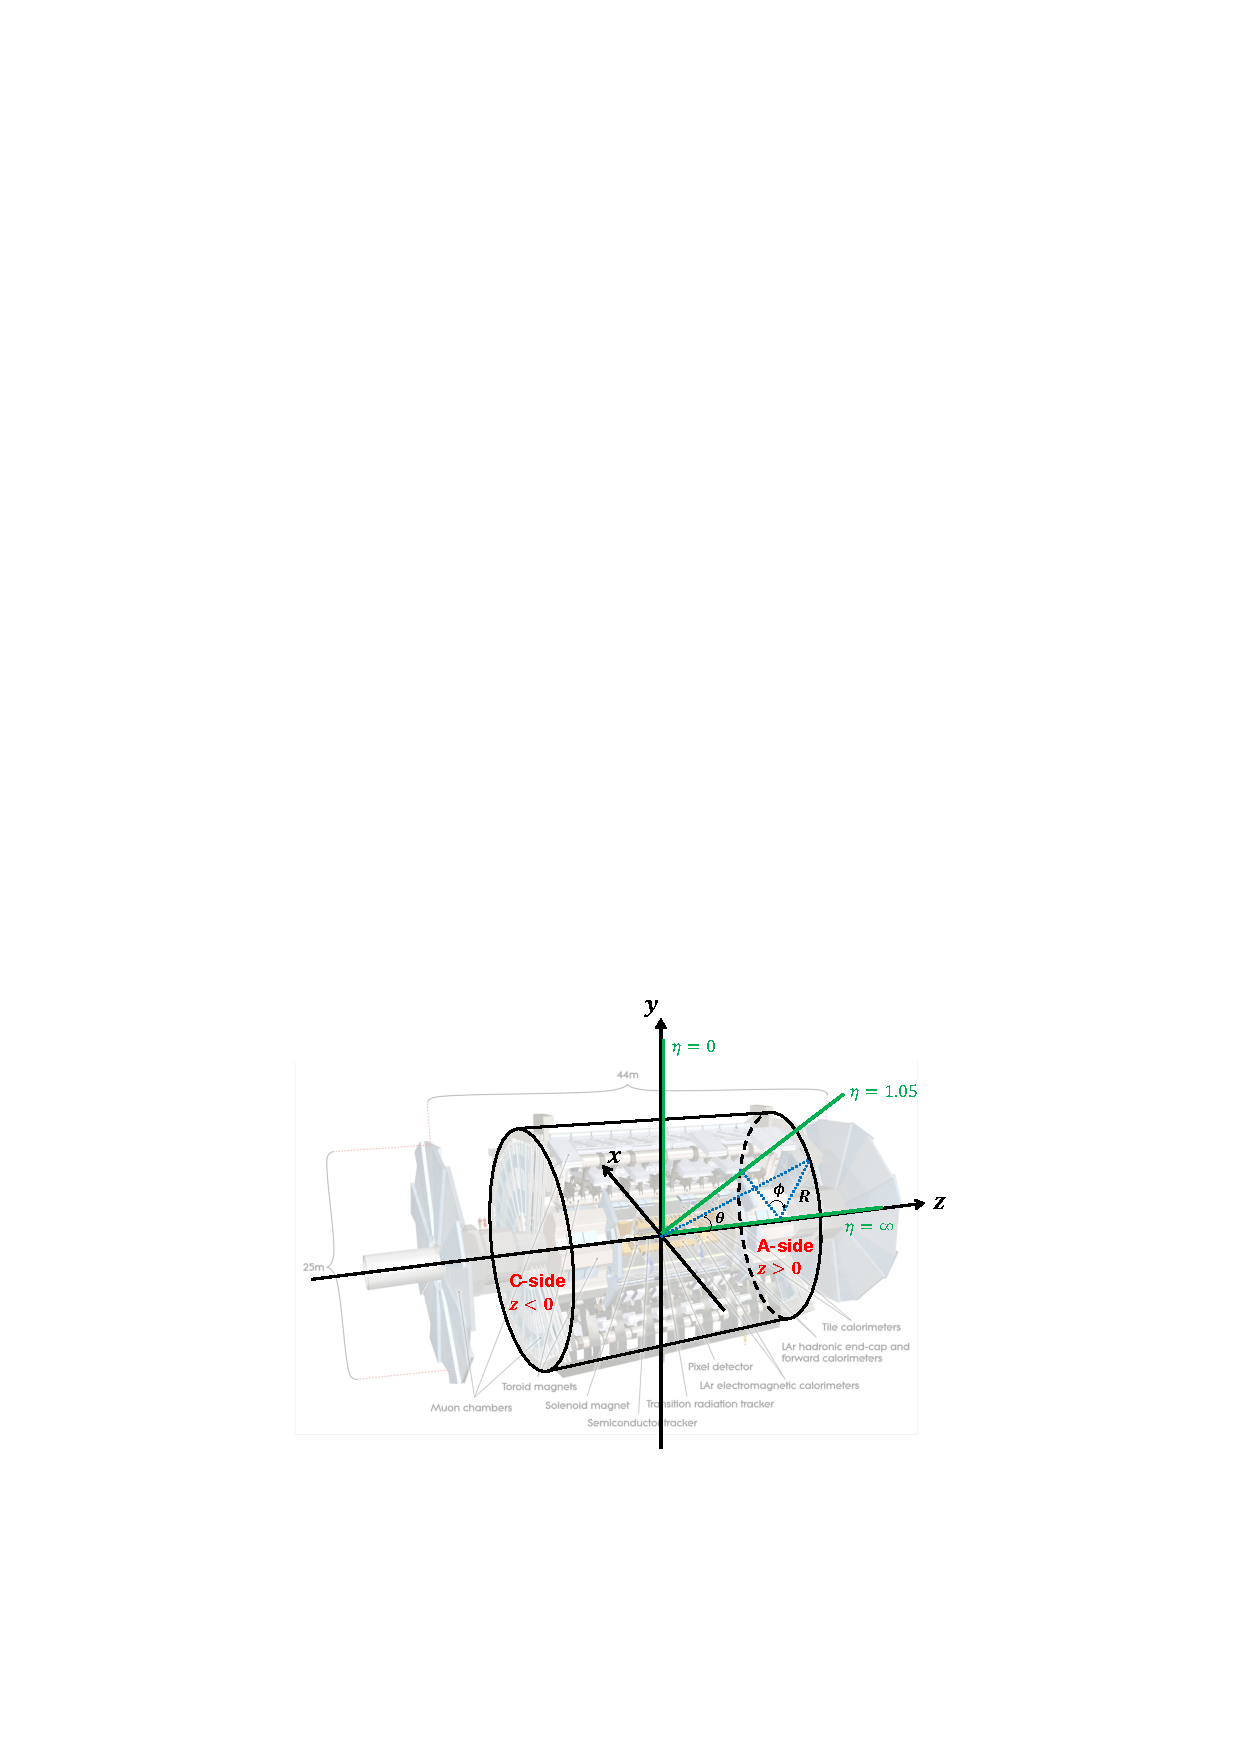
\includegraphics[width=16cm]{fig/Intro/ATLAScordination.pdf}
\caption[ATLAS検出器における座標系]{ATLAS検出器における座標系}
\label{ATLAScordination}
\end{figure}



\begin{figure}
    \begin{minipage}[b]{.5\linewidth}
    \centering
        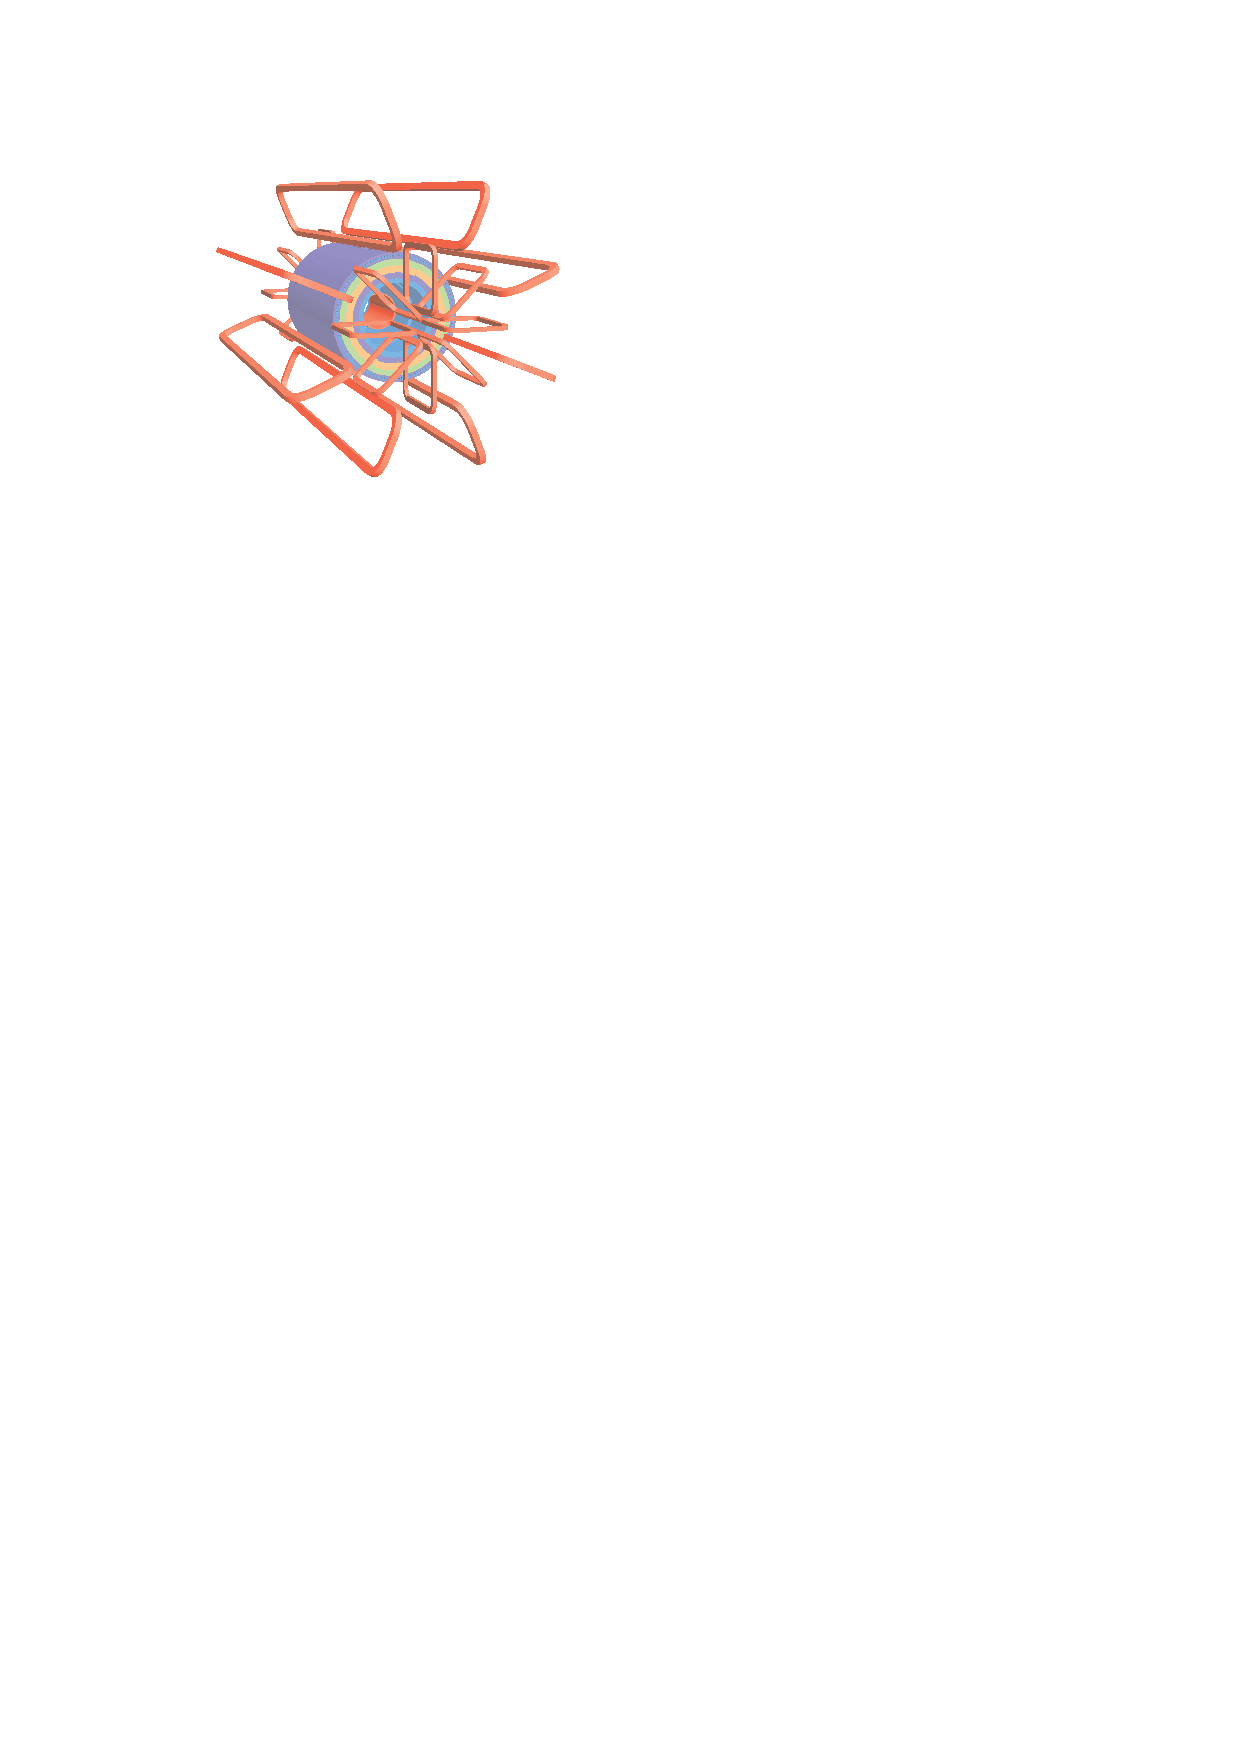
\includegraphics[height=5cm]{fig/Intro/ATLASmagnet.pdf}
        \subcaption*{(a)超伝導磁石の設置}
        \end{minipage}%
    \begin{minipage}[b]{.5\linewidth}
        \centering
        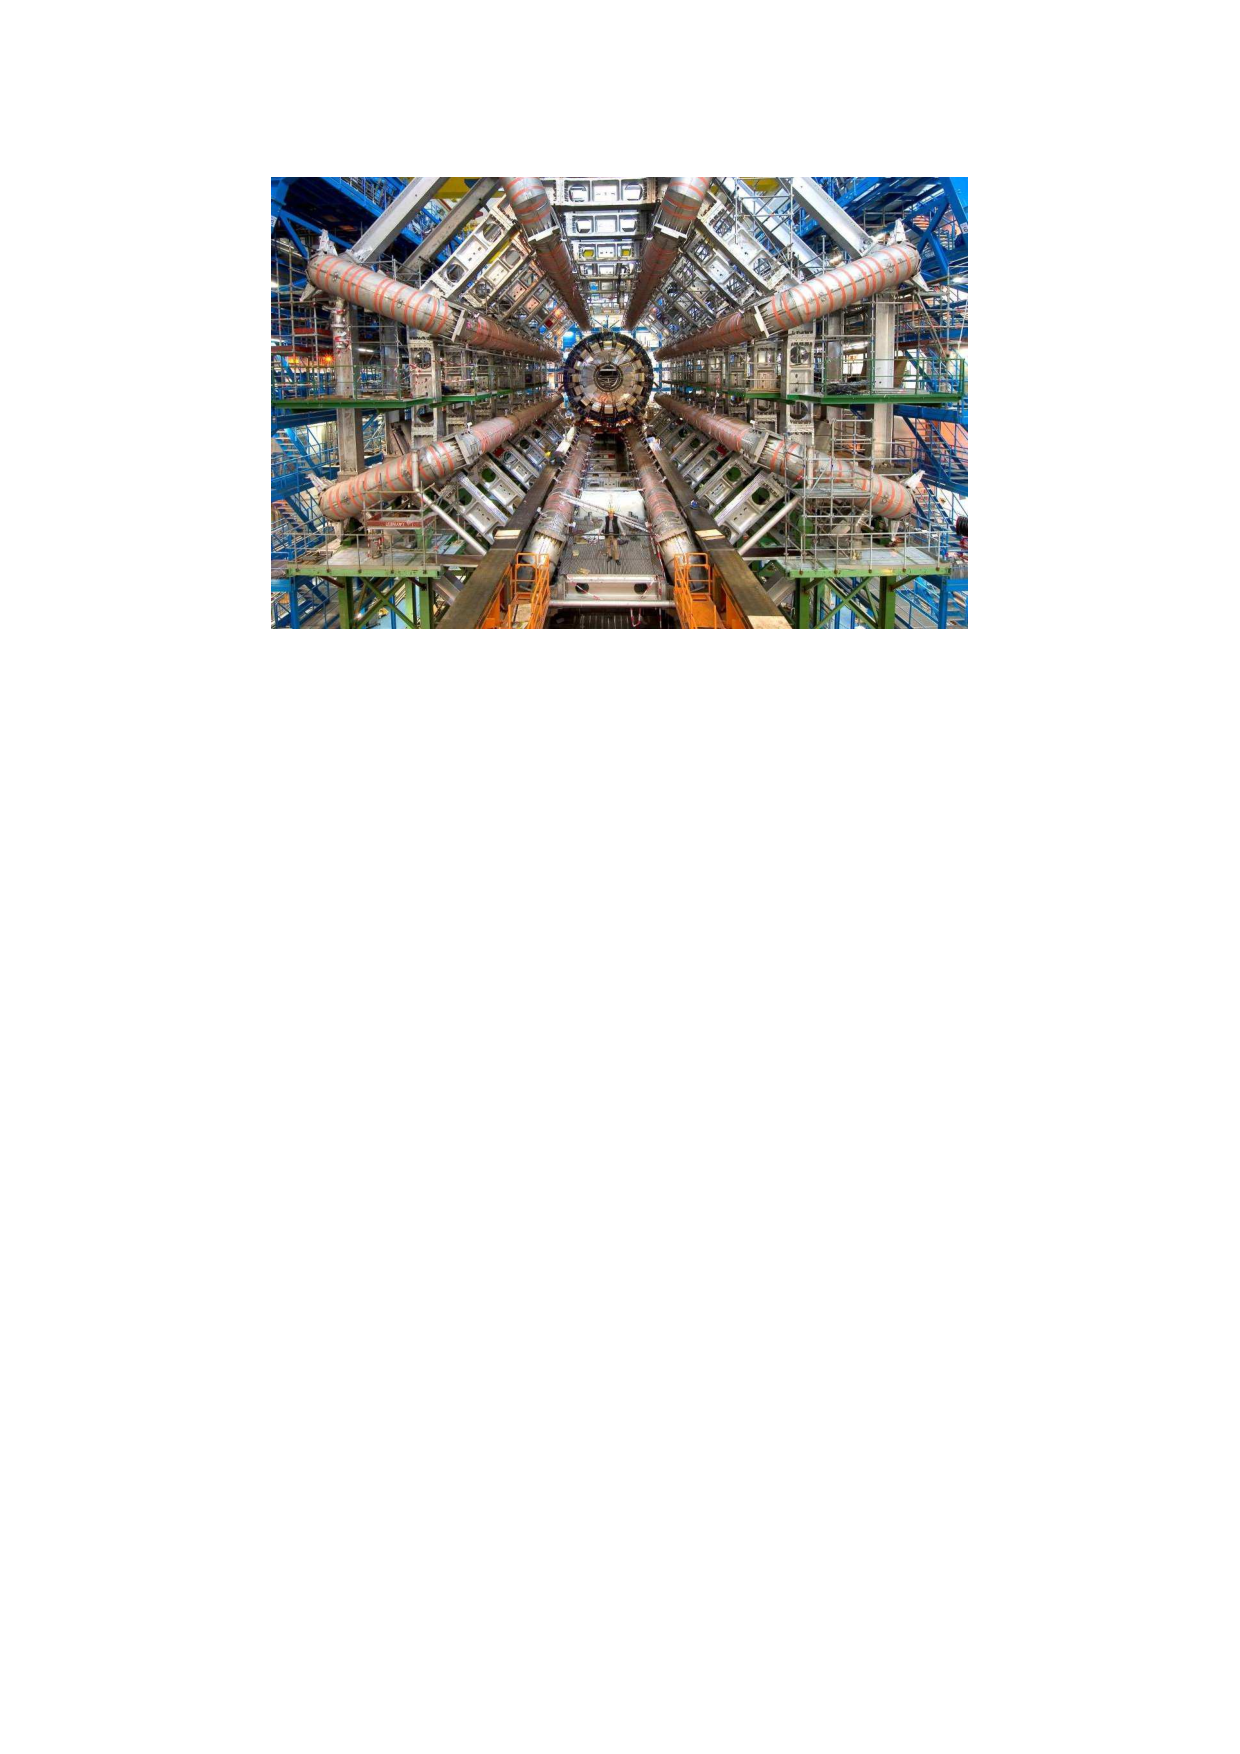
\includegraphics[height=5cm]{fig/Intro/ATLAStroido.pdf}
        \subcaption*{(b)ATLAS検出器のbarrel toroid magnet}
    \end{minipage}%
    \caption[異なる画像形式の比較]{異なる画像形式の比較。(a) PDF形式。拡大しても綺麗であり、文字も検索やコピーができる。(b) PNG形式。拡大するとビットマップ画像であることが分かる。文字を選択できない。(c) JPEG形式。PNGに比べ、JPEG圧縮特有のブロックノイズ、モスキートノイズが発生しており非常に汚いことが分かる。}
\end{figure}

\begin{figure} 
    \centering
    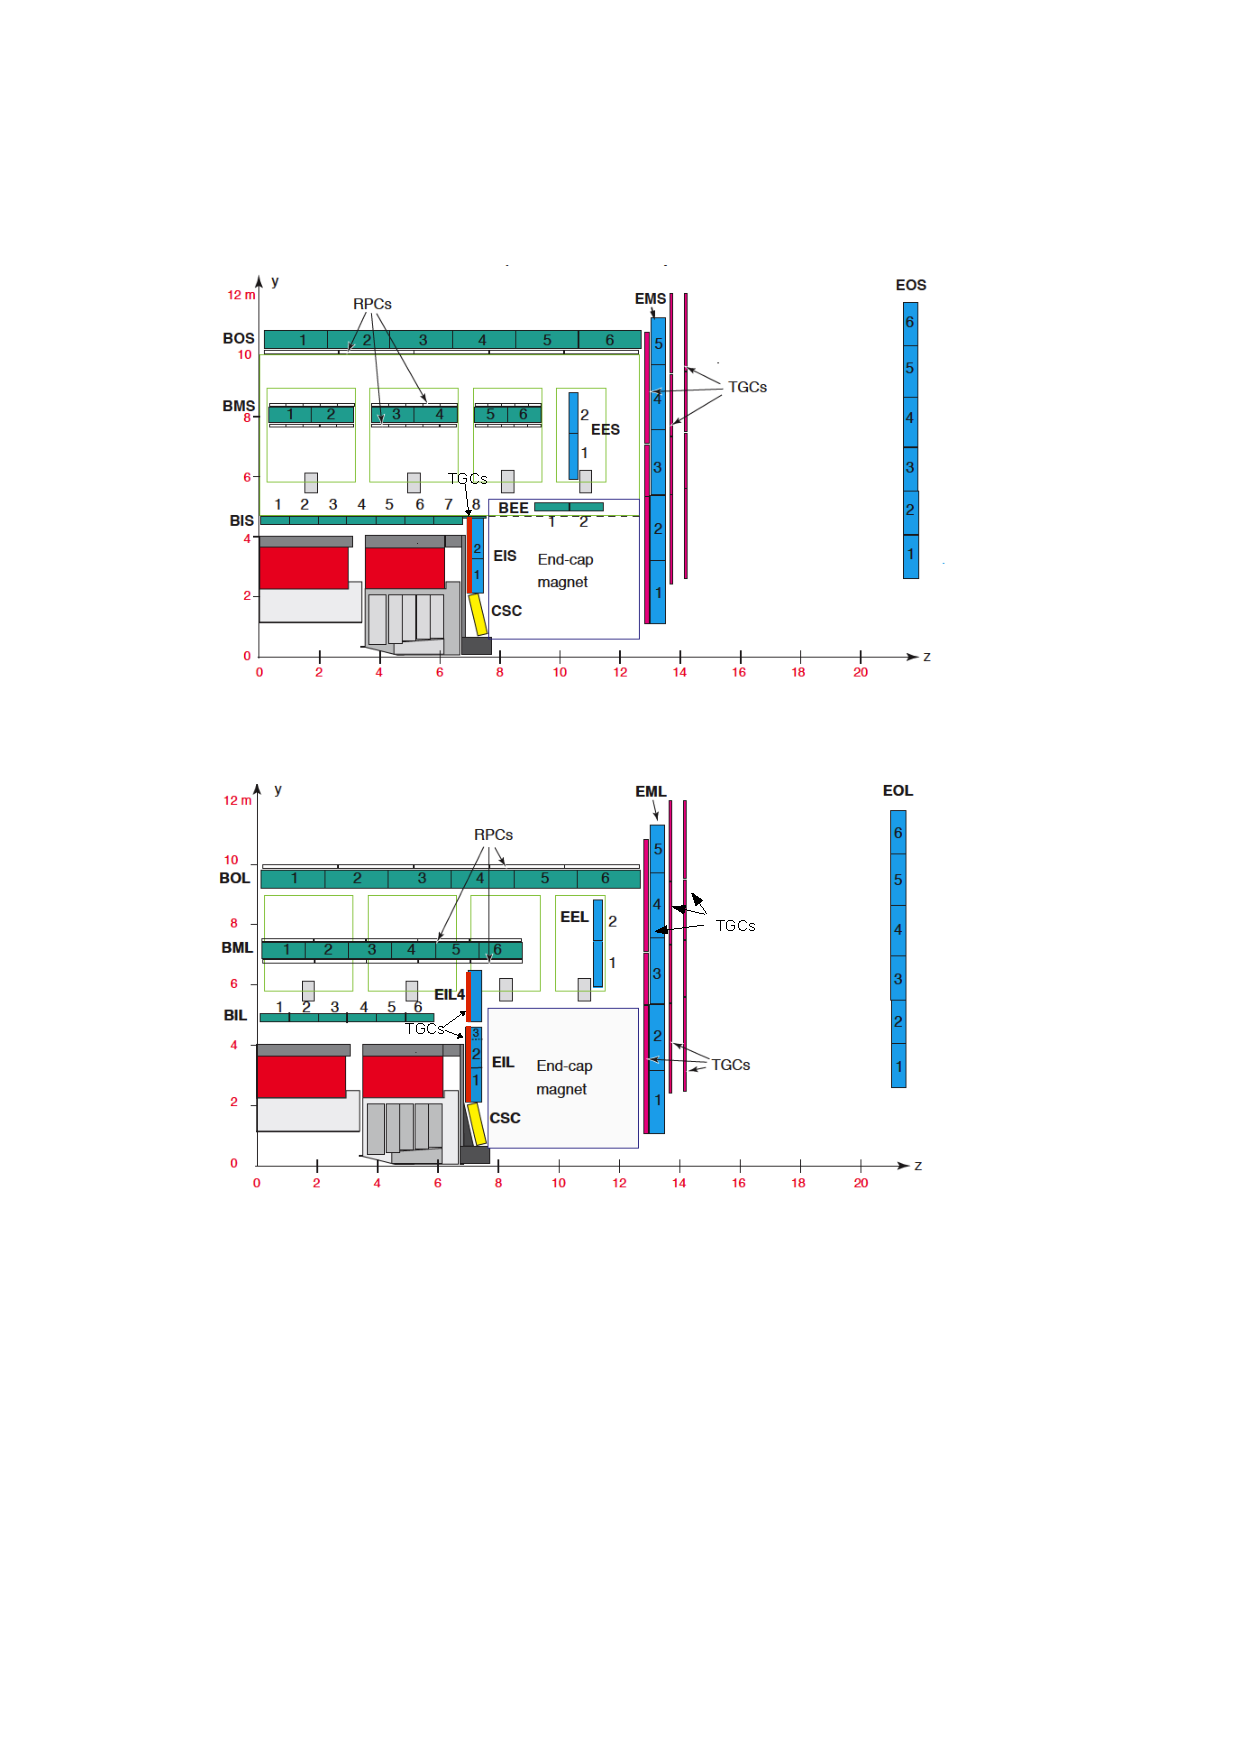
\includegraphics[width=16cm]{fig/Intro/Muonspectrometer.pdf}
    \caption[高輝度LHC-ATLAS実験でのミューオンスペクトロメーターの断面図]{高輝度LHC-ATLAS実験でのミューオンスペクトロメーターの断面図\cite{tdr_phase2muon_2017017}}
    \label{Muonspectrometer}
\end{figure}
    


\section{ATLAS実験におけるTDAQシステム}
\label{sec_TDAQ}

\section{TGC検出器トリガーシステム}
\label{sec_TGCtrigger}

\subsection{TGC検出器トリガー原理}
\label{subsec_TGCtriprinciple}

\subsection{Run3でのTGCトリガーシステム}
\label{subsec_run3trig}

\subsection{高輝度LHC-ATLAS実験でのGCトリガーシステム}







